\newcommand{\B}{{\boldsymbol b}}

\chapter{Advanced QHD Parameter Sets}\label{ch: advanced}

\section{Introduction}

This chapter will explore a more general QHD formalism and will implement two parameter sets: FSUGold and NL3. In this formalism, additional meson fields, in the form of the rho meson field, and higher order coupling terms for the familiar meson fields, the scalar and vector meson fields, will be included. Furthermore, the equation of state will be made more realistic by including constraints for beta-equilibrium, including the addition of two lepton species (electrons and muons).

This chapter will not go into the same detail as \autoref{ch: qhd1} for its derivations. These were beyond the scope of the project and not the main intention; instead, it was most important to practice calculating an EOS and to reproduce the results in \autocite{diener_2008}.

% crust and equilibrium conditions; not ``complete'' eos here


\section{Equations of Motion and RMF Simplifications}\label{sec: adv, eom}

In this chapter, we work with a more general Lagrange density for QHD
\begin{align}
    \Lag & = \psi \bqty{\gamma^\mu\qty(i\p_\mu -g_vV_\mu - \frac{g_\rho}{2}{\boldsymbol\tau}\cdot {\boldsymbol b}_\mu)-(M-g_s\phi)}\psi\nonumber\\
    & \quad + \frac{1}{2}\p_\mu \p^\mu \phi - \frac{1}{2}m_s^2\phi^2 - \frac{\kappa}{3!}(g_s\phi)^3 - \frac{\lambda}{4!}(g_s\phi)^4 \nonumber\\
    & \quad - \frac{1}{4} V^{\mu\nu}V_{\mu\nu} + \frac{1}{2} m_\omega^2 V^\mu V_\mu + \frac{\zeta}{4!}(g_v^2 V^\mu V_\mu)^2 \nonumber\\
    & \quad - \frac{1}{4} \B^{\mu\nu} \B_{\mu\nu} + \frac{1}{2}m_\rho^2 \B^\mu \cdot \B_\mu + \Lambda_v (g_v^2 V^\mu V_\mu)(g_\rho^2 \B^\mu \cdot \B_\mu),
\end{align}
where
\begin{align*}
    V_{\mu\nu} \Def \p_\mu V_\nu - \p_\nu V_\mu, \quad
    \B_{\mu\nu} \Def \p_\mu \B_\nu - \p_\nu \B_\mu.
\end{align*}
These fields are identical to those in \autoref{ch: qhd1}, with the addition of the $\B$ field and additional coupling constants: $\phi$ represents the scalar meson field, $V_\mu$ the vector meson field, $\psi$ the baryon field, and $\B = (b^\mu_1, b_2^\mu, b_3^\mu)$, the three isospin components of the rho meson field. ${\boldsymbol\tau} = (\tau_1, \tau_2, \tau_3)$ is called the \textit{isospin} operator, defined in terms of the Pauli Matrices; see \autocite[pp. 72-73]{diener_2008} for more details. 

The additional coupling constants arise from allowing higher order terms in $V_\mu$ and $\phi$ into the Lagrange density. For the scalar field, $\phi$, this includes $\kappa$ and $\lambda$, the third and fourth order self coupling constants, respectively. For the vector meson field, $\zeta$ is the self coupling constant. Finally, the coupling between the rho meson and vector meson fields is quantified by $\Lambda_v$.

Intuitively, including additional meson fields and higher order couplings will make the Lagrangian more accurate, while at the same time more complicated. These extra terms better model the meson exchange and the interactions between the fields, but at the expense of computability.

For this system, we once again introduce the relativistic mean field (RMF) simplifications, where we take all fields to be their average values. These simplifications are
\begin{align}
    \phi &\goesto \bra{\Phi} \phi \ket{\Phi} = \expval{\phi} \Def \phi_0, \\
    V^\mu & \goesto \bra{\Phi} V^\mu \ket{\Phi} = \expval{V^\mu} \Def \delta^{\mu 0} V_0,\\
    \B^\mu & \goesto \bra{\Phi} b^\mu_i \ket{\Phi} = \expval{b^\mu_i} \Def \delta^{\mu 0} \delta_{i3} b_0.
\end{align}

The simplifications for $\phi$ and $V^\mu$ are identical to those in \autoref{sec: qhd1, rmf}. However, the simplifications are more complicated for $\B^\mu$. Because $\B^\mu$ contains three components, each with four components of their own, we write $\B^\mu$ as $b_i^\mu$, where the lower index only takes the values $i \in \Bqty{1,2,3}$. By \autocite[p. 74]{diener_2008}, only the $i=3$ component of $\B^\mu$ has a non-vanishing expectation value, so we add an extra Kronecker-delta to enforce this condition. 

Once again, we also must form the expectation values of the baryon operators $\bar\psi$ and $\psi$ with the various other operators in the Lagrange density. These give
\begin{align}
    \bar\psi\psi &\goesto \bra{\Phi}\!:\!\psi\psi\!:\!\ket{\Phi} = \expval{\bar\psi\psi},\\
    \bar\psi\gamma^\mu \psi &\goesto \bra{\Phi}\!:\!\psi\gamma^\mu\psi\!:\!\ket{\Phi} = \expval{\psi\gamma^0\psi},\\
    \bar\psi\gamma^\mu\tau_i\psi &\goesto \bra{\Phi}\!:\!\psi\gamma^\mu\tau_i\psi\!:\!\ket{\Phi} = \expval{\psi\gamma^0\tau_3\psi}.
\end{align}

We once again follow the procedure described in \autoref{ch: qhd1}. We first apply the Euler-Lagrange equations in \eqref{eqn: ELE}, as we did in \autoref{sec: qhd1, eom derivation}. This yields four equations of motion for the cases of $\varphi \in \Bqty{\phi_0,V_0,b_0,\bar\psi}$. We immediately apply the above RMF simplifications; each kills terms with derivatives and introduces expectation values containing the baryon operators, like those in the above equations. From here, there is once again a rigorous mathematical procedure for calculating the forms of these expectation values, which is beyond the scope of this paper. After substituting the expressions for these expectation values, the three equations of motion for the meson fields reduce to, as shown in \autocite[p. 79]{diener_2008}
\begin{align}
    \phi_0 & = \frac{g_s}{m_s^2}\bqty{\frac{1}{\pi^2} \pqty{\int_0^{k_p} \dd{k} \frac{k^2 m^*}{\sqrt{k^2 + m^{*2}}} + \int_0^{k_n} \dd{k} \frac{k^2 m^*}{\sqrt{k^2 + m^{*2}}}} -\frac{\kappa}{2}(g_s\phi_0)^2 -\frac{\lambda}{6}(g_s\phi_0)^3 }\label{eqn: adv, phi0}\\
    V_0 & = \frac{g_v}{m_s^2} \bqty{\rho_p + \rho_n - \frac{\zeta}{6}(g_v V_0)^3 - 2 \Lambda_v (g_vV_0)(g_\rho b_0)^2}\label{eqn: adv, V0}\\
    b_0 & = \frac{g_\rho}{m_\rho^2} \bqty{\frac{1}{2}(\rho_p - \rho_n) - 2\Lambda_v(g_vV_0)^2(g_\rho b_0)}\label{eqn: adv, b0}
\end{align}

There is an analogous way to determine equations for $\epsilon$ and $P$ from the Lagrange density for this more advanced system as in \autoref{sec: qhd1, rmf}. After doing so, we once again apply the RMF simplifications and determine the values of the expectation values. This gives the forms of $\epsilon$ and $P$ in (9.20) in \autocite[p. 79]{diener_2008}. However, as mentioned in the introduction, this EOS takes into account the effects of leptons, too, namely electrons and muons. This requires the inclusion of two additional integrals over the Fermi-momenta of both the electrons and muons, given on \autocite[p. 92]{diener_2008}. These forms of $\epsilon$ and $P$ are given below.
\begin{align}
    \epsilon = & +\frac{1}{2}m_s^2\phi_0^2 + \frac{\kappa}{3!} (g_s\phi_0)^3 + \frac{\lambda}{4!}(g_s\phi_0)^4 - \frac 12 m_\omega^2V_0^2 - \frac{\zeta}{4!}(g_vV_0)^4 \nonumber\\
    & - \frac 12 m_\rho^2 b_0^2 - \Lambda_v(g_vV_0)^2(g_\rho b_0)^2 + g_vV_0(\rho_n + \rho_p) + \frac{1}{2} (\rho_p-\rho_n) \nonumber\\
    & + \frac{1}{\pi^2}\bqty{\int_0^{k_p} \dd{k} k^2 \sqrt{k^2 + m^{*2}} + \int_0^{k_n} \dd{k} k^2 \sqrt{k^2 + m^{*2}}}\nonumber\\
    & + \frac{1}{\pi^2} \bqty{\int_0^{k_e} \dd{k} k^2 \sqrt{k^2 + m_e^2} + \int_0^{k_\mu} \dd{k} k^2 \sqrt{k^2 + m_\mu^2}}\label{eqn: adv, eps}\\
    P = & -\frac{1}{2}m_s^2\phi_0^2 - \frac{\kappa}{3!} (g_s\phi_0)^3 - \frac{\lambda}{4!}(g_s\phi_0)^4 + \frac 12 m_\omega^2V_0^2 + \frac{\zeta}{4!}(g_vV_0)^4 \nonumber\\
    & + \frac 12 m_\rho^2 b_0^2 + \Lambda_v(g_vV_0)^2(g_\rho b_0)^2 \nonumber\\
    & + \frac{1}{3\pi^2}\bqty{\int_0^{k_p} \dd{k} \frac{k^4}{\sqrt{k^2 + m^{*2}}} + \int_0^{k_n} \dd{k} \frac{k^4}{\sqrt{k^2 + m^{*2}}}}\nonumber\\
    & + \frac{1}{3\pi^2} \bqty{\int_0^{k_e} \dd{k} k^2 \sqrt{k^2 + m_e^2} + \int_0^{k_\mu} \dd{k} k^2 \sqrt{k^2 + m_\mu^2}} \label{eqn: adv, p}
\end{align}

% The equations for $\phi_0,V_0,b_0,\epsilon$, and $P$ given above will be used, in conjunction with the constraint equations from \autoref{sec: adv, constraints}, to calculate the equation of state.


\section{Equilibrium Conditions}\label{sec: adv, constraints}

As described above, this chapter will explore a more realistic equation of state by including additional constraints to enforce beta-equilibrium. This section will describe those constraints and how they fit into the model.

To begin, we define the number density for a species of particle $\rho_x$ and its corresponding Fermi-momenta by the equations
\begin{align}\label{eqn: adv, k to rho}
    \rho_x = \frac{k_x^3}{3\pi^2} \quad\Longleftrightarrow\quad k_x = (3\pi^2\rho_x)^{1/3}.
\end{align}
This will be a useful result that will be used constantly throughout \autoref{sec: adv, gen}.

In the \autoref{ch: qhd1}, our loop variable was $k_f$; however, in this calculation, we choose to use $\rho$, the total baryon number density, as the loop variable. Due to the above equation, we can directly relate these two quantities as needed.

At any iteration of the loop variable $\rho$, the number densities of baryons must stay constant; thus, we have
\begin{align}\label{eqn: adv, conservation of number density}
    \rho = \rho_n + \rho_p,
\end{align}
where $\rho_n$ is the number density of the first species, neutrons, while $\rho_p$ is the number density of the second species, protons. That is, throughout the iteration, the total number density of protons and neutrons must stay constant. This condition comes from the decay of neutrons into protons, electrons, and anti-neutrinos called beta-decay.

There is a reverse process, however, where a proton and electron combine to form a neutron and a neutrino. This process is possible and likely due to the high energies of electrons present in the extreme conditions within a neutron star. These ``competing'' processes work until \textit{beta-equilibrium} is reached, where, in a given iteration, $\rho_p$ and $\rho_n$ are such that $\epsilon$ is minimized. If we define the chemical potential as
\begin{align}\label{eqn: adv, chemical potential def}
    \mu_x \Def \pdv{\epsilon}{\rho_x}, 
\end{align}
for the $x$th chemical potential, the condition for beta-equilibrium can therefore be written as
\begin{align}\label{eqn: adv, beta equilibrium, mus}
    \mu_n = \mu_p + \mu_e.
\end{align}
Using a convenient result in (10.7) on \autocite[p. 90]{diener_2008}, we can rewrite this more generally as
\begin{align}\label{eqn: adv, beta equilibrium}
    \sqrt{k_n^2 + m^{*2}} = \sqrt{k_p^2 + m^{*2}} + g_\rho b_0 + \sqrt{k_e^2 + m_e^2}.
\end{align}
This expression is found by calculating the chemical potentials $\mu_n, \mu_p,$ and $\mu_e$ by differentiating \eqref{eqn: adv, eps} with respect to different number densities by \eqref{eqn: adv, chemical potential def} and substituting into \eqref{eqn: adv, beta equilibrium, mus}.

Furthermore, within neutron stars, there is a third reaction in which a muon decays into an electron, a neutrino, and an anti-neutrino. Once the energies are large enough, and muon states have become populated, the muon formation and decay must be in equilibrium; this is quantified by the equality of their chemical potentials
\begin{align}\label{eqn: adv, equil of electrons and muons}
    \mu_\mu = \mu_e,\quad \mu_e  = \sqrt{k_e^2 + m_e^2}, \quad \mu_\mu  = \sqrt{k_\mu^2 + m_\mu^2}.
\end{align}

Our final constraint is charge conservation; because muons and electrons have equal charges, opposite that of protons, this constraint takes the form
\begin{align}\label{eqn: adv, charge conservation}
    \rho_p = \rho_e + \rho_\mu \goesto k_p = \pqty{k_e^3 + k_\mu^3}^{1/3}.
\end{align}

These four constraint equations, \eqref{eqn: adv, conservation of number density}, \eqref{eqn: adv, beta equilibrium}, \eqref{eqn: adv, equil of electrons and muons}, and \eqref{eqn: adv, charge conservation}, in conjunction with the equations of motion in \eqref{eqn: adv, phi0}, \eqref{eqn: adv, V0}, and \eqref{eqn: adv, b0} must be solved concurrently. This will be described in detail below.

\section{Numerical Generation of the Equation of State}\label{sec: adv, gen}

Within this section, important code blocks will be included for reading convenience; however, any line numbers will reference the complete code sample given at the conclusion of this paper in \autoref{ch: advanced code}.

This section will describe the procedure for numerically calculating the equation of state from the constraint equations in \autoref{sec: adv, constraints} and the equations of motion in \autoref{sec: adv, eom}, and then the following process for computing $\epsilon$ and $P$.

In lines 1-53 of the file, the values of the constants for the two analyzed parameter sets, NL3 and FSUGold, are implemented. This includes the initialization of the coupling constants and the masses of the fields. 

\begin{lstlisting}
@njit
def k_from_rho(rho):
    return (3*np.pi**2*rho)**(1/3)

@njit
def rho_from_k(k):
    return k**3/(3*np.pi**2)
\end{lstlisting}

At this point, we define the two above functions. These are implementations of the equation (and its inverse) present in \eqref{eqn: adv, k to rho}. Of note is the \code{@njit} ``decorator'' from the Numba library present on both of these functions. Numba is a Python library that has tools for improving the speed of Python code through ``just-in-time'' (jit) code compilation. In these situations, where the code is simple and repeatable, with predictable datatypes, providing this decorator can make these functions much faster; whenever possible, we applied it to functions that we were writing. 

We next had to decide how to solve our set of seven coupled equations efficiently. Specifically, we have the constraint equations: the conservation of baryon number density \eqref{eqn: adv, conservation of number density}, the beta equilibrium condition \eqref{eqn: adv, beta equilibrium}, the equality of the muon and electron chemical potentials \eqref{eqn: adv, equil of electrons and muons}, charge equality \eqref{eqn: adv, charge conservation}, followed by the equations of motion: the $\phi_0$ equation \eqref{eqn: adv, phi0}, the $V_0$ equation \eqref{eqn: adv, V0}, and the $b_0$ equation \eqref{eqn: adv, b0}. At each step in the process, we must solve \textit{all} of these equations at the same time to determine a solution. Fortunately, there are numerous solvers implemented to solve such a system by minimizing a set of residuals; in our case, we chose the SciPy solver titled \code{least\_squares}.

\begin{lstlisting}
def ns_system(vec, rho):
    rho_n, rho_p, rho_e, rho_mu, phi0, V0, b0 = vec

    k_n = k_from_rho(rho_n)
    k_p = k_from_rho(rho_p)
    k_e = k_from_rho(rho_e)
    k_mu = k_from_rho(rho_mu)

    mu_mu = np.sqrt(k_mu**2 + m_mu**2)
    mu_e = np.sqrt(k_e**2 + m_e**2)
    
    mstar = (M - g_s*phi0)

    f = lambda k: (k**2*mstar)/np.sqrt(k**2 + mstar**2)
    p_int, p_err = quad(f,0,k_p)
    n_int, n_err = quad(f,0,k_n)

    return np.array([
        # conservation of baryon number density
        rho - (rho_n + rho_p), 
        # beta equilibrium condition
        np.sqrt(k_n**2 + mstar**2) - (np.sqrt(k_p**2 + mstar**2) + g_rho*b0 + np.sqrt(k_e**2 + m_e**2)),
        # equilibrium of muons and electrons
        mu_mu - mu_e, 
        # charge equilibrium
        k_p - (k_e**3 + k_mu**3)**(1/3), 
        # phi0 equation
        phi0 -  g_s/(m_s**2) * (1/np.pi**2 * (p_int + n_int) -kappa/2 * (g_s * phi0)**2 - lmbda/6 * (g_s * phi0)**3), 
        # V0 equation
        V0 - g_v/m_omega**2 * (rho_p + rho_n - zeta/6 * (g_v * V0)**3 - 2*Lmbda_v*(g_v * V0)*(g_rho * b0)**2),
        # b0 equation
        b0 - g_rho/m_rho**2 * (1/2 * (rho_p - rho_n) - 2*Lmbda_v*(g_v * V0)**2*(g_rho * b0))
    ])
\end{lstlisting}

Therefore, we created a function for the evolution of the system of equations included in \autoref{sec: adv, eom} and \autoref{sec: adv, constraints} called \code{ns\_system}, shown above. This function was to be passed to \code{least\_squares} as the evolution function. \code{least\_squares} requires a function whose argument is a vector\footnote{Our function has two parameters; the first is a vector, and the second is a parameter $\rho$ necessary for determining the rest of the values within this evolution equation. The SciPy solver (which will be shown later) allows for additional arguments to be passed by using the \code{args} keyword and passing a list of arguments in the order they should be passed; this is how the value of $\rho$ is injected to \code{ns\_system} throughout its calls.} (tuple) containing all the variables whose solution we are looking for, with a return value of an array containing the \textit{residuals} of the equations in the system. The solver then minimizes the system of residuals as a system and returns a vector containing the value of the variables that \textit{caused} that minimum condition, the solution that we are looking for.

Our \code{ns\_system} function, therefore, was written to satisfy these conditions. First, the variable \code{vec} contains the seven variables whose values we want to determine: $\rho_n, \rho_p, \rho_e, \rho_\mu,$ $\phi_0,$  $V_0,$ and $b_0$. Importantly, by decision, we decide to determine the number densities ($\rho_x$) of the different species of particles present, and not the corresponding Fermi-momentas ($k_x$). From the known information, then calculate the Fermi-momentum of each particle, the chemical potentials $\mu_\mu$ and $\mu_e$, the reduced mass $m^*$, and the integrals present in the $\phi_0$ equation; once again, the integrals are calculated numerically using the SciPy \code{quad} function. Then, each of the equations mentioned above are implemented as a residual by subtracting the right-hand side of the equation to find an expression equal to zero. During the minimization, the residual is squared and minimized, and the resulting solution values of the vector are returned by \code{least\_squares}.

After the definition of \code{ns\_system}, we implement another sister function named \code{ns\_sy-} \code{stem\_no\_muons}. There comes a point during the evolution when the muon Fermi-momenta, defined by $k_\mu = \sqrt{\mu_\mu^2 - m_\mu^2},$ becomes imaginary; at this point, no more muons are produced, and the evolution should no longer include muons at all. In this function, the parameter \code{vec} does not include $\rho_\mu$ and does not contain the residual $\mu_\mu = \mu_e$, the equivalence of chemical potentials between electrons and muons. Once $k_\mu$ becomes close enough to zero, we begin evolving this function instead; this switch will be specifically outlined below.

\begin{lstlisting}
def eps(vec):
    if len(vec) == 6:
        rho_n, rho_p, rho_e, phi0, V0, b0 = vec
        rho_mu = 0
    else:
        rho_n, rho_p, rho_e, rho_mu, phi0, V0, b0 = vec
    
    # omitted ...
\end{lstlisting}

After this point, we define both the $\epsilon$ and $P$ functions; the beginning of the $\epsilon$ function is shown above, while the $P$ function is omitted, as it has the same initial form and simply performs some different calculations in its body. Importantly, both functions are equipped to handle both the muon and non-muon cases; this is shown by the lines above. If the vector only contains six variables, it means that muons are not currently being produced, so the muon number density $\rho_\mu$ should be zero; otherwise, we should unpack the vector as expected. In the body of the function, in the ``omitted'' section, both functions carry out numerical integrations and simple numerical calculations to return the values of $\epsilon$ and $P$.

\begin{lstlisting}
rho_exp = np.linspace(-1, -5, 5000)
x0 = [.2, .2, .2, .2, .2, .2, .2]

n = -1
for i,exp in enumerate(rho_exp):
    rho = 10**(exp)

    if x0[3] <= 1e-12:
        n = i
        break

    sol = least_squares(ns_system, x0, args=[rho], method='lm')

    x0 = sol.x
    output.write(f'{eps(x0):.16e}, {P(x0):.16e}\n')

x0 = x0[0], x0[1], x0[2], x0[4], x0[5], x0[6]

for i in range(n, len(rho_exp)):
    # no muon section ...
\end{lstlisting}

At this point, we are ready to calculate the equation of state. We begin with an initial guess \code{x0}; by trial and error, we found an adequate value to be $.2$ for all variables. Then, we begin looping through our exponents\footnote{To easily work on a logarithmic range, we simply iterate over an exponent linearly, and each point, just raise 10 to that exponent.}, beginning at -1. In each iteration of the loop, we first calculated the $\rho$ value, our total baryon number density, using this exponent. Towards the bottom, we create \code{sol}, the solution to our \code{least\_squares} minimization, with our $\rho$ value as an argument and the \code{x0} value as an initial guess. Then, we extract the solution, set it as our initial guess for the next iteration, and write the $\epsilon$ and $P$ values to file for the current solution.

In the middle of the function, we have a break condition; this is the point at which the muons are no longer produced. \code{x0[3]} is the current $\rho_\mu$ value, and once that drops below a threshold, in this case \SI{e-12}{}, we break from the current \code{for} loop. At this point, we form a new initial condition, without the previous value of $\rho_\mu$ (\code{x0[3]} is no longer present) and then begin iterating through the remainder of the exponent values. The omitted section, ``no muon section,'' performs the same procedure as described above, however with the evolution function \code{ns\_system\_no\_muons}. After this second loop is completed, the equation of state will be tabulated in a file.

At this point, we solve the TOV equations using the NL3 parameter set in order to compare to the plot given on \autocite[p. 117]{diener_2008}. This plot is for a neutron star in beta-equilibrium with no crustal effects included. Our reproduction is given below in \autoref{fig: NL3 M vs R}.

\begin{figure}[h!]
    \centering
    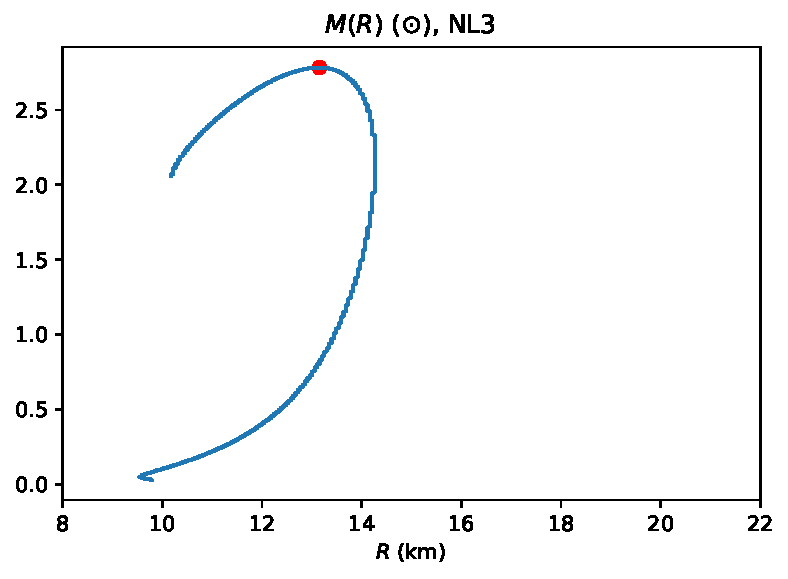
\includegraphics[width = .75\textwidth]{images/adv/r_analysis,NL3-2.pdf}
    \caption{The $M(R)$ plot for the NL3 parameter set for comparison to Fig. A.3 on \autocite[p. 117]{diener_2008}}
    \label{fig: NL3 M vs R}
\end{figure}

Our plot matches up perfectly with the one given in \autocite{diener_2008}, demonstrating the validity of our code and calculation. Originally, our goal was to continue by calculating crustal effects and adding them to this equation of state, which is valid for the inner core. We then would have compared to the plots given on \autocite[p. 102]{diener_2008}, both for NL3 and FSUGold.

\begin{figure}[h!]
    \centering
    \begin{subfigure}{.5\textwidth}
        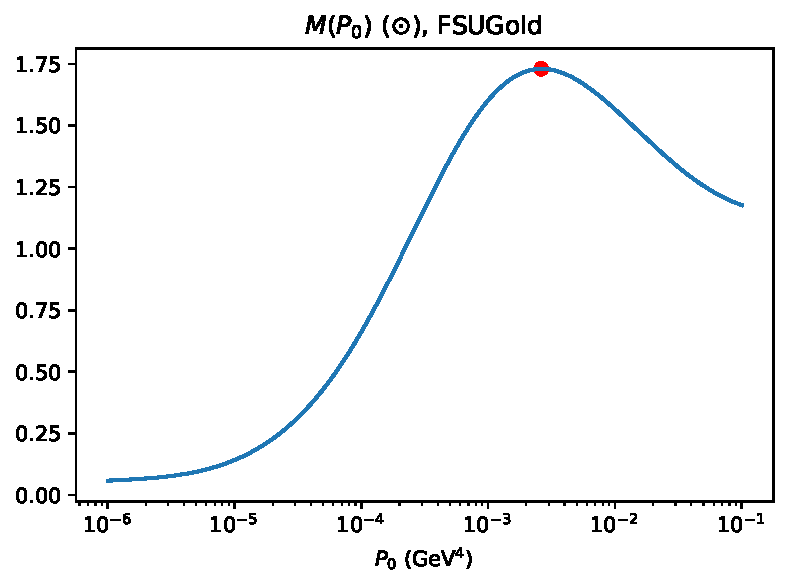
\includegraphics[width=\textwidth]{images/adv/p0_analysis,FSUGold.pdf}
    \end{subfigure}%
    \begin{subfigure}{.5\textwidth}
        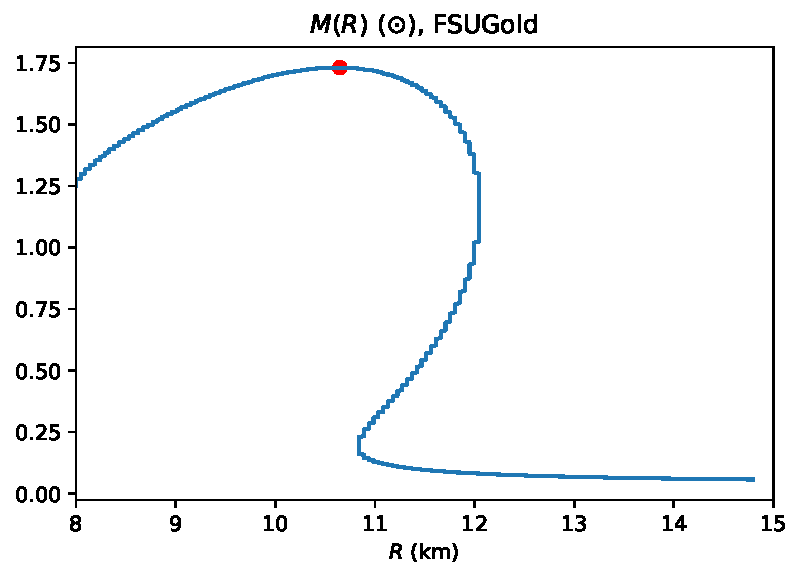
\includegraphics[width=\textwidth]{images/adv/r_analysis,FSUGold.pdf}
    \end{subfigure}
    \caption{The mass-pressure curve (left) and mass-radius curve (right) for the FSUGold equation of state given in \autocite{diener_2008}.}
    \label{fig: fsugold mass radius pressure}
\end{figure}

\begin{figure}[h!]
    \centering
    \begin{subfigure}{.5\textwidth}
        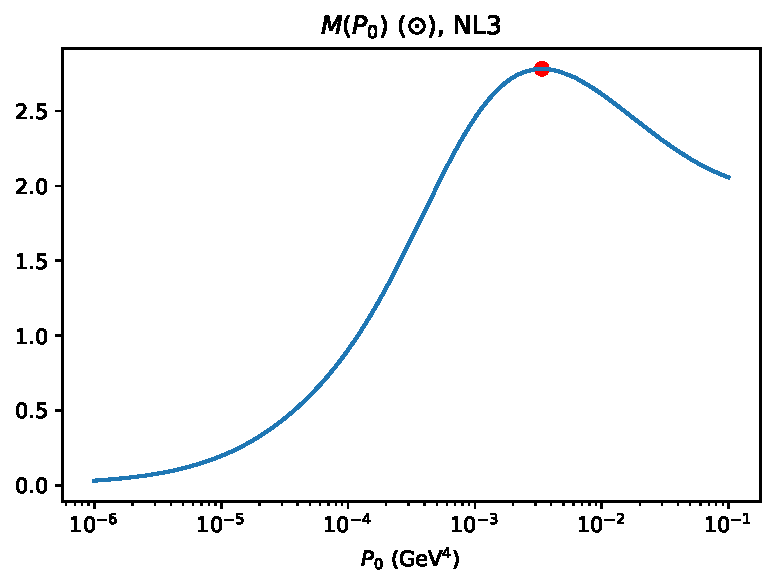
\includegraphics[width=\textwidth]{images/adv/p0_analysis,NL3.pdf}
    \end{subfigure}%
    \begin{subfigure}{.5\textwidth}
        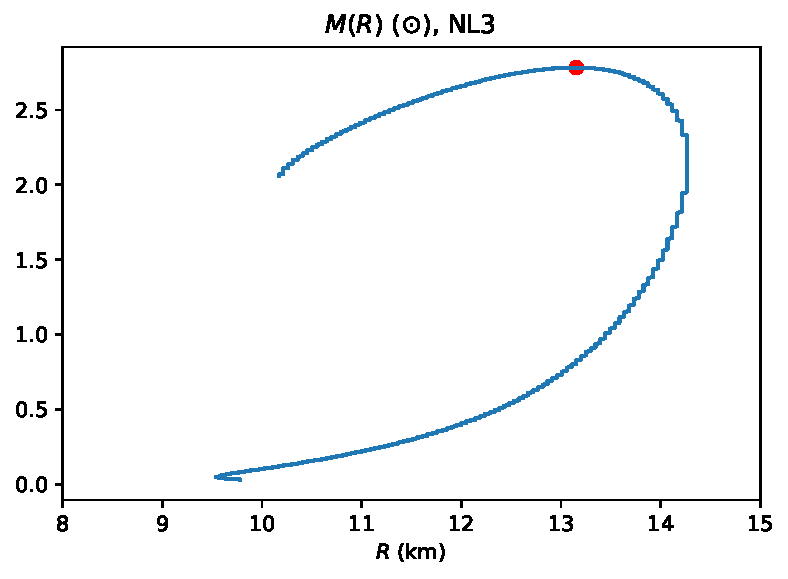
\includegraphics[width=\textwidth]{images/adv/r_analysis,NL3.pdf}
    \end{subfigure}
    \caption{The mass-pressure curve (left) and mass-radius curve (right) for the NL3 equation of state given in \autocite{diener_2008}.}
    \label{fig: nl3 mass radius pressure}
\end{figure}

While the implementation of the EOSs for NL3 and FSUGold are not considered complete, as they simply include descriptions of the inner crust, we still calculated the critical mass and radius from the TOV equations to present and to compare the results to those in the QHD-I EOS from \autoref{ch: qhd1}. From \autoref{fig: fsugold mass radius pressure}, we get predictions for FSUGold: $M_\text{max} = \SI{1.73}{\odot}$ and $R_\text{max} = \SI{10.6}{km}$. Similarly, \autoref{fig: nl3 mass radius pressure} gives the following predictions for NL3: $M_\text{max} = \SI{2.78}{\odot}$ and $R_\text{max} = \SI{13.2}{km}$. These values are much closer to those of the realistic, analytic EOSs of the SLy family given in \autoref{fig: tov, all eos analyses}. This is a testament to the additional steps taken within their derivation: the inclusion of the rho-meson field, and the additional constraints present to satisfy beta-equilibrium. These steps make the calculated equations of state much more realistic. In comparision, the predictions that QHD-I makes ($M_\text{max} = \SI{6.1}{\odot}$ and $R_\text{max} = \SI{42.1}{km}$) seem quite unrealistic.